\documentclass[nolof,digital]{fithesis3}
\thesissetup{faculty=fi}
\thesissetup{author=Bc. Lukáš Tyrychtr,id=422294, departmentEn = Faculty of Informatics, programmeEn = Applied Informatics, fieldEn = Applied Informatics, assignment = {}}
\thesissetup{type= mgr}
\thesissetup{title=Feel the streets - a visually impaired user access to OSM maps}
\thesissetup{keywords = {visually impaired, navigation, accessibility, Open Street Map, usability}}
\usepackage[english]{babel}
\usepackage{alltt}
\usepackage{listings}
\usepackage{csquotes}
\usepackage[hidelinks]{hyperref}
\usepackage[style=ieee,sorting=nty,block=ragged]{biblatex}
\renewbibmacro*{bbx:savehash}{} %disabling dashing
\addbibresource{bibliography.bib}
\usepackage{tabularx}
\usepackage{placeins}
\usepackage{tabu}
\usepackage{algorithm2e}
\SetAlCapSkip{3mm}
\usepackage{graphicx}
\graphicspath{{./images/}}
\thesislong{abstract}{

}
\thesissetup{advisor=Ing. Milan Brož\, Ph.D.}
\thesislong{thanks}{
I would like to thank all my thesis advisors for their beneficial tips and for their time in general. I would also like to thank all the testers, and, with his permission, special thanks go to Martin Jozífek, who helped track many nasty issues and dedicated a lot of his time which allowed the application to be in much better shape than it was before.
}
\thesisload
\setcounter{tocdepth}{2}
\begin{document}
\chapter{Introduction}
Being a visually impaired individual poses many challenges in day-to-day life. One of the more obvious ones is the inability to navigate in unknown areas relatively easily.

When a sighted person is faced with the challenge of going through an unknown route, he can see it quite well most of the time, or, when the route is more complex, he can use a map. However, when visually impaired, this approach is not easy either.

It is true that the development of technology brought various possibilities like usage of smartphones, however, creating an application which can present a map is not something trivial even for the audience of sighted people. There are also tactile approaches, however they pose other challenges.

The goal of this thesis is to present the currently viable choices for map presentation and to introduce a new application which can help visually impaired people to explore their surroundings in as much detail as the source data allow.

In the second chapter, this thesis explores the choices for a visually impaired person related to map exploration and navigation.

The third chapter presents Feel the Streets, the main reason for the existence of this thesis. It explores the motivations, implemented features, used technologies, and the history which led to the current state. It also talks about some issues which were encountered during the development.

Having a potentially useful application is not enough, however. Every potential user has different needs and expectations, so it is important to discover what exactly the users think. To accomplish this goal, a study was performed withing a group of visually impaired people. The main goal of the study was to discover any usability issues which might exist. This study is described in chapter four.

The fifth chapter summarizes the conclusions and presents the future work which is necessary to make the application more successful than a one-person project for hobby purposes. The last part of the thesis presents the appendices which did not fit into the structure but are nonetheless useful in understanding the results of the work.
\chapter{Map presentation approaches}
Using a map is one of the more common approaches when a person wants to learn an unknown area. However, it poses a challenge for visually impaired people because it is necessary to represent the map somehow. It is possible to describe the area verbally, which is commonly done. However, sometimes a more map-like approach is helpful as well. So this chapter describes the various approaches which can be used to present maps to visually impaired people, mainly focusing on tactile maps and various applications for smartphones and desktop operating systems.
\section{Printed maps}
According to \parencite{orientation_aids_from_foundations}, tactile maps are considered the most effective representation for information related to an unknown space. On the other hand, this kind of map is nontrivial to create and often requires manual work.

To help in creating tactile maps, Mapy.cz now allows export to a format which is suitable for tactile printing \parencite{mapycz}. The export contains essential elements like street outlines, some buildings, and other related features. This system uses data from Seznam.cz for the Czech Republic and OpenStreetMap data for the rest of the world.

Another system allowing to create a tactile map from OpenStreetMap data is \parencite{tactile_osm_maps}. It also allows to specify the starting point of the map and also the zoom level used for rendering. The rendering tries to show important features for the visually impaired, such as tactile paving.
\section{Mobile phone apps}
As smartphones started being ubiquitous in the population of visually impaired people, some special applications for the respective operating systems were created. Also, the standard navigation applications developers did not completely forget accessibility, so this section describes the most common applications used by visually impaired people on the two major smartphone operating systems.
\subsection{Google maps}
Google Maps \parencite{googlemaps} is a map application created by Google. It started as a web application and was also ported to various smartphone operating systems, including Android and iOS. The application supports displaying the map, searching for nearby places in various categories, navigation features, and other related functions, such as adding place reviews and location sharing between users. Google had a somewhat longer time to get good coverage of the world, so the data are generally regarded as better than Apple's, but it processes more personal data from the users \parencite{mapcomp}.

From a visually impaired user perspective, the interface is quite accessible, except for the area displaying the actual graphical map. The navigation functionality is also usable well, thanks to quite specific voice prompts along the planned route.
\subsection{Apple maps}
Apple Maps \parencite{applemaps} is a mapping application used by Apple in their operating systems. The basic features - map exploration, searching by name or category, exploring the graphical map, are there as well.

For visually impaired users, the application is fully accessible. It even allows the visually impaired user to look around the map to get a feel about the spatial relationships of streets. This feature allows a visually impaired user to slide the finger on the screen and be notified about the current street under it.
\subsection{BlindSquare}
BlindSquare \parencite{blindsquare} is an application primarily for visually impaired users on the iOS operating system. The application uses Foursquare and OpenStreetMap to help the user determine its current location and to find out what is nearby.

The application supports reporting the current address based on the user's GPS location, reporting nearby crossings and other venues. It also allows searching by name or category. The application can also automatically report new nearby objects. BlindSquare also supports adding bookmarks specified by the user. For navigation to the point of interest BlindSquare uses third-party applications on the user's device.
\subsection{Lazarillo}
Lazarillo \parencite{lazarillo} is somewhat similar to BlindSquare. However, Lazarillo is available for Android and iOS operating systems. The basic BlindSquare features like near places discovery, search, favorite places are there. In addition to these features, Lazarillo allows you to set a tracked object and monitor your distance to it in real-time. It also has some business-related features for indoor navigation, sharing accessibility-related information, and it also has related features to help the users navigate.
\subsection{Where Am I}
Where am I \parencite{whereami} is an Android application allowing the user to determine his location, copy his GPS coordinates and calculate distances between arbitrary two locations.
\subsection{Naviterier}
Naviterier \parencite{naviterier} is an application that provides specially tailored routes for visually impaired users. These routes contain many more details (crossing and corner descriptions, curb information, and similar hints), allowing the visually impaired to walk the planned route with fewer surprises than with a traditional navigation application. The application is available as a web application that can show the entire planned route and as a mobile application for Android and iOS.

Because planning for visually impaired users requires much more details than is available in OpenStreetMap or Google Maps, the application has good enough data coverage only in Prague. The best results can only be achieved in the city's center, where the application has the most complete data coverage. In the center, the application uses data from the ROUTE4ALL platform \parencite{route4all}. In the rest of the supported areas, it uses traditional map data and human curation of the details needed for navigation purposes of the visually impaired.
\subsection{OsmAnd}
OsmAnd \parencite{osmand} is an offline application for Android and iOS supporting offline map browsing and navigation. It uses OpenStreetMap as its source of data and supports map viewing, searching for points of interest, adding favorite places, and can also optionally display specialized overlays.

The accessibility of the application on iOS, according to personal experiences, is not ideal, there are some wrongly labeled buttons and related minor issues, but the application is usable, at least route planning and similar features. According to a talk with a friend, the situation on the Android operating system is much better; there, all elements have correct labels.
\subsection{Dotwalker}
Dotwalker \parencite{dotwalker} is an Android application helping visually impaired users look around and navigate along a route. The user can view nearby points in various categories or add its own and import a route either from directions from Google Maps or OpenStreetMap. The application supports offline operations except for the import operations from online sources.

The application also shows the current compass direction and allows sharing the current location between users.
\subsection{Right Hear}
RightHear \parencite{righthear} is an application for Android and iOS that is primarily designated to help visually impaired people navigate buildings. That is accomplished using a network of Bluetooth beacons that contain information relevant to the user in a particular place. The application also supports outdoor navigation. It very likely uses OpenStreetMap data because the website specifies that it uses open-source map data.
\subsection{Ariadne GPS}
AriadneGPS \parencite{ariadnegps} is a paid iOS application that allows a visually impaired user to explore his surroundings and save points of interest and navigate to them or be notified when the points are in range. The application allows the user to explore spatial relationships on the map by touching the map area. By default, the exploration mode only shows streets, addresses, and intersections. However, the user can turn on a mode that shows more features, for example, parks. A cursory personal analysis shows that AriadneGPS uses both Apple Maps and Google Maps as its sources. Unfortunately, it does not allow displaying more details about the places and does not allow searching for known points of interest (shops, restaurants, and similar).
\section{Desktop apps}
Despite the Usage of desktops being quite common, not many navigation-related applications are accessible on desktop operating systems. The web interfaces of various services can be used with various degrees of success. However, the functional features are limited to route searches.

This section thus describes the single application mentioned in the research.
\subsection{Plánovač tras Google}
This Czech-only application \parencite{ptg} allows the users to do a route search using Google's route search API. The route is then displayed as an accessible list of individual route steps. The search can be constrained by the mode of transport, whether public transport can be used, and similar parameters. The application also allows displaying the known places around a location using Google's places API.
\section{Summary}
As was shown in this chapter, navigation applications for smartphone operating systems are usable. The user can perform basic operations like searching for a route, browsing near by places and in some cases it is also possible to get a basic understanding of the spatial relationships of the area shown by the map. However, presenting the actual map is nonetheless a challenge. The data source is often a commercial offering, which might be an issue for some users.
\chapter{Feel the streets} \label{ref:fts}
As can be seen from the previous chapter, when a visually impaired user wants to browse a map on a desktop operating system accessibly and use features more advanced than route planning, the choices are not good, or the applications are somewhat hard to use.

That is the reason why Feel the Streets was born, and I spent quite a lot of time writing it. Therefore this chapter describes the application features and then describes the development history and the various architectural changes along the way.

The main reasons for writing Feel the Streets were that none of the applications mentioned in the previous chapter could provide the desired map exploration experience on a desktop operating system. To add to that, making the application cross-platform could expand the userbase as well. And the last reason was that the presentation of OpenStreetMap data for a visually impaired person was not much helpful, so this application changes that and makes the data accessible.
\section{Feature overview}
From the user's perspective, Feel the Streets is a desktop application that, when launched, allows the user to browse OpenStreetMap maps without sight.
\subsection{Area selection}
After startup, the application presents a list of the available areas from which the user can choose one which he wants to browse. This window is shown in the below figure.
\begin{figure}[h]
\caption{The area selection window of Feel the Streets}[h]
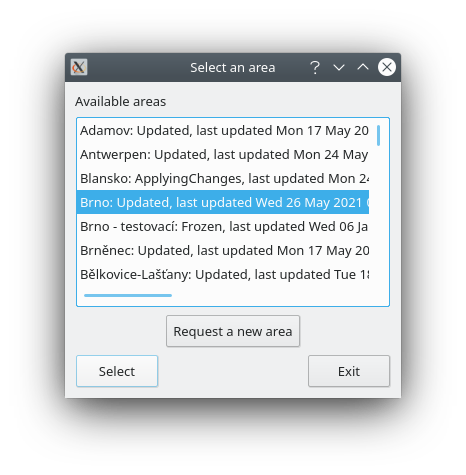
\includegraphics{fts-areas}
\end{figure}
The areas list is usually retrieved from the Feel the Streets server, so it includes all the available areas. Still, when there is no network connectivity, the locally available areas are shown instead.

The areas list shows the area's name, last modification, and creation times formatted according to the user's locale preferences, the area size, and its state. The state represents the status of the area's database, and it usually reports that the area is updated. Other states exist as well, namely states for an area that is just being created, for which we are just now retrieving the incremental changes, or we are applying them. A  concept of frozen areas exists, these areas can be downloaded, but after creation, no changes are applied to them, which is helpful for research reproducibility.

From the area selection window, the user can also request an area that is not yet available. If he does so, he is prompted for the area's name, and if there are multiple candidates, he is then offered the list of the areas to specify which one he actually means. This selection process is helped by including all the area properties in the candidate details window.

By selecting an area, a set of steps starts. If the selected area is not yet downloaded to the user's computer, the download is performed. If it is, the application checks for all the changes which occurred to the area between the last check and now and applies them. After these steps, the user ends up in the main window.
\subsection{The main window}

The application's main window is seemingly simple - just an empty window with a menubar on top. Despite this, it is the central piece of the user interface of the application. It is shown, along with the nearby objects window, which is described in the next section, in the following figure.
\begin{figure}[h]
\caption{The main window of Feel the Streets along with the nearby objects window}
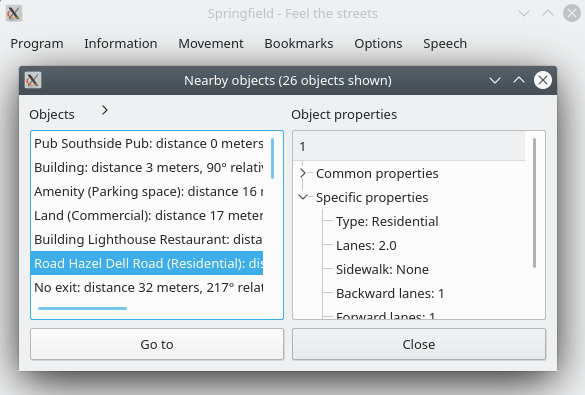
\includegraphics{feel-the-streets}
\label{fig:fts}
\end{figure}

This is the window where the actual map exploration occurs. Because of that, it contains all the relevant commands.

The first group of commands allows the user to move in the environment. It allows him to do a forward and backward step. It also allows him to turn around in 5 and 90-degree increments, change his direction by a given amount, and jump to a particular set of GPS coordinates.

The next group of commands allows the user to determine his location. He can request a summary of it, or he can request a more detailed view of it using the nearby objects window, which is described in a subsequent subsection. The user can also request a list of nearby objects. Usually, some objects are not considered (like routes and similar relatively big objects), but the user can request the location of nearby objects without ignoring these.

The next group of commands provides various additional information about the application's state. These additional commands include reporting the user's current GPS coordinates, his direction or allowing him to browse the history of spoken messages during the current application run; the speech history is not saved between restarts of the application.

There is also a set of commands which allows toggling some of the application settings.
\subsection{Search}
The application also allows performing searches in the data. There are two search facilities.

The first is a simple search based on a partial name match. The user can enter a part of the desired name, and every object with that particular substring in its name tag is returned.

When the name search is not sufficiently detailed, the user can use the advanced search. In this mode, he is first required to select which kind of object he wants to search - everything with an address, shops, buildings, and more. After the selection, he can specify additional conditions based on the selected entity's fields. For strings, it is possible to use exact or partial matches. For numbers, all the usual operators are available. The user can specify any number of conditions which are then combined into the final query as if there was a logical and operator between them. This window is shown in the next figure.
\begin{figure}
\caption{Advanced search of amenities filtered to universities}
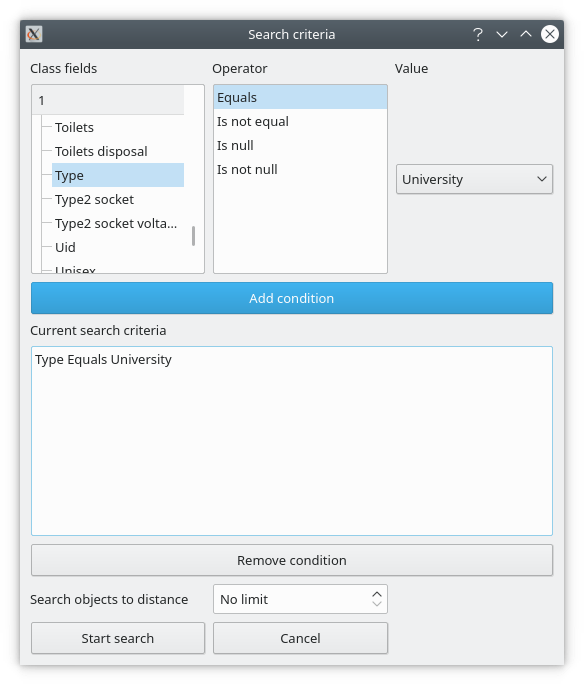
\includegraphics{fts-amenity-university}
\end{figure}

In both of the search modes, the results are displayed using the same window which is used for the nearby objects.
\subsection{The objects list window}
This window is used for displaying a list of objects. This list can come from a nearby query, a search, or it can be a result of a parent/child query as well. It is shown in figure \ref{fig:fts}.

The window shows a list of objects represented as short descriptions of them. In each case, it contains the entity class of it and some details (like the name, amenity type) for some of the classes. In addition, when an object is selected, all the properties (basically OpenStreetMap tags when not counting some renaming of the tag names) are displayed. In addition, the user can expand a part of the properties that contain the revision information, including the last changed date, the user who did the change, the changeset number. This section also shows the object's id, which is the OpenStreetMap id prefixed by a letter (n for nodes, w for ways, and r for relations) to allow the user to communicate precisely which object might require some fixes, for example.

The window also allows performing additional actions on some of the objects. The more useful of these actions include opening a website related to the object or opening its Wikipedia entry. The actions also allow viewing the parents (e. g., the relations or ways that contain the given object) or the object's children. The parent object might be helpful to, for example, determine the railway line for a part of its tracks.
\subsection{Navigational sounds}
During navigation, the application plays some sounds to help the user visualize the relationships between the object positions and distances.

As a first clue, it plays sounds for some objects, currently for land areas, shops, and trash cans. These sounds are played on the correct 3d cartesian coordinates, so the relationships between them are preserved.

In addition to these sounds, the application also plays sounds for crossings.

Both of these groups of sounds can be turned on and off if desired.
\subsection{Automatic announcements of interesting objects}
To help the user discover potentially interesting objects, the application automatically announces some of the nearby entities. This announcement uses a much shorter distance than the scan of the nearby object. For now, the object is announced regardless of its reachability, so it might be possible that an object is announced even if it is behind some other buildings.

These announcements can, of course, be turned off using a configuration option.
\section{Technical overview}
This section describes the currently used technologies which are used by the Feel the Streets client and server. The technologies have changed quite extensively during the development, so the Development history section then presents the various choices which were made during the lifetime of the application.

As of now - commit f316b17d63, which can be found along with the entire development history at \parencite{fts_repo}, the application is comprised of two major components and some supporting libraries and utilities. The major components are the client and server applications, respectively. They share the area database access layer through python bindings.
\subsection{The client}
The client is the main application with which all the users interact. It handles downloading of the area databases, applying updates, and browsing the respective areas.

The client application is written in the Python programming language \parencite{python}. Python was chosen mainly because it was familiar and had good library support for all the subsystems.

For the user interface, the Qt library \parencite{qt} is being used as it has the best cross-platform accessibility story despite some mainly Windows-specific issues.

For the sound engine, the client application uses OpenAL and the HRTF extension. That means that the OpenAL Soft library \parencite{openalsoft} is required.
\subsection{The server}
The server mainly handles the management of area databases. It handles the area creation requests from the clients and helps the clients keep their local databases updated, and it also creates a list of changes that the clients can download afterward.

It is written in the Rust programming language \parencite{rust}, mainly for speed and memory usage reasons. The static typing helped the development as well, and it was not so uncommon to find an error that a statically typed language would prevent.

For storage of the area databases, the SQLite3 library \parencite{sqlite} is used. To perform the needed geospatial queries, the SpatiaLite extension \parencite{spatialite} is being used.

For communication with the client application, the server exposes an HTTP API for area lists, download requests, and similar functionality. 

For storing the area changes, a RabbitMQ \parencite{rabbitmq} server is used. It allows keeping the queue semantics quite easily. The clients do not have full administrative access to the Rabbitmq server when connecting, they are limited by an access control list, and the connection is also secured using Transport layer security.

To keep the number of additional components as low as possible, RabbitMQ is also used for background task storage and for background task scheduling. The scheduling uses the message's time to live, and it instructs RabbitMQ to put the message to the ready messages queue after the TTL expires.

The server uses compression extensively to minimize the storage requirements. The main savings are by compressing the individual area database changes before putting them in the Rabbitmq queue. The compression uses the Zstdandard compression algorithm \parencite{zstd} which allows, among other things, to use a pre-trained compression dictionary for compression, which gives much better results than compressing the individual messages on its own - it gave an improvement of at least of 50\% in message sizes on average.

To help discover new kinds of amenities and another enum like tags during the processing of areas and to find other anomalies in the assumed schema of the OSM data (type violations, unknown properties, and others), a record of these events is logged during the operation and it is stored for further analysis. The processing application, however, is not implemented yet. Or, more correctly, the features were lost during the Rust rewrite, which is described in the following section.
\subsection{The shared library}
The handling of area databases is actually implemented in a shared library, called osm\_db, which is called from the server code and from Python as well. To allow calling the library from Python, creating a binding library was necessary. Fortunately, by using the Pyo3 Rust library \parencite{pyo3}, that effort was relatively straightforward. The Python library does not expose the entire public API of osm\_db, only the parts which the client application requires, which means basically the complete query API and a way to apply database changes.
\subsection{The administrative command-line application}
To allow performing some maintenance and related tasks for the server, such as requesting clients to perform redownload of an area, making a rename of a field, and some more actions, a command-line application that interacted with the server-side area databases and queues was implemented.
\section{Development history} \label{ref:devhistory}
This section presents the development history of Feel the Streets, the various approaches used, and their advantages and disadvantages. It also mentions some of the accessibility issues, which are further described in the issues encountered along the way section. This section does not describe each commit of the Feel the Streets repository. It mentions only the more important ones.
\subsection{The beginnings}
The first commit of the Feel the Streets project occurred on the 18th of August 2017. At this time, the application's GUI used the wxWidgets library \parencite{wx}, and there was no server component. The area database access was handled using the SQLAlchemy library, and it used the sqlalchemy's table inheritance features, so there was a separate table for each entity class.

The initial implementation of the database update logic was added in the next commit.

In commit 683215bbe1, the search functionality was added.
\subsection{Table inheritance removal}
It turned out, mainly because of the search functionality, which required quite huge joins, and it managed to cross the Sqlite3's maximum column count for a query result as well, that the approach which used a separate table for each entity was not sustainable. As a result, in commit 3a02c10710, the area database structure was changed, so all the entities were stored in a single table with the entity properties stored in a JSON object. This storage approach survived the current version of Feel the Streets, except for some minor modifications. The application representation stayed largely similar, the entity classes kept a Python class, but these classes existed only for the application and used the Pydantic data validation library.
\subsection{Bookmarks appear}
In commit dbb8a71b2b, the initial support for bookmarks was added. The bookmarks were stored in the area database, which was changed in commit 30d56506d9 to allow safe area redownloads. To accomplish this, a database stored in the user's application data directory was introduced. The last change of the bookmark representation occurred in commit 49bc7331ae, which added the user's direction when creating the bookmark that was not stored before.
\subsection{The server is born}
Because of the need to update the area databases incrementally and not downloading them each time, commit 8fe9a7548f introduced a concept of semantic changes of OSM objects. The following commit introduced the server component and moved the update logic there, and in commit fab61d9f61, the server API was introduced.

When the server API was in place, commit d791a35bad allowed the users to select a map. 

And some commits later, when the server's capability to run an update of all area databases was deemed stable enough, commit b2fd5c4943 implemented the client-side of area updates.
\subsection{Object actions}
In commit 62a1454247, the framework for executing actions on objects was introduced. Some commits later, the Wikipedia and wiki data open actions were implemented along with other website-like things which could be opened, like the RUIAN details of a Czech building.
\subsection{The rustification efford}
Because of the languages used, the server memory consumption and speed were not ideal. To improve the situation, a quite drastic measurement was taken starting from commit 67b194c60a. The entire server component was a small piece at a time rewritten into Rust. That required rethinking the way how the entity properties and generator property mappings are stored, so the server used a few YAML files to store the entity classes and their properties, the enums inherent in the data, and the translation transformations. The server rewrite effort was merged into master in commit 42a9e4762a.

In commit b5b9ea13a1, the creation of python bindings of osm\_db has started. That allowed getting rid of the python entity classes, and access to the area database was unified at last.

Along with the rewrite, the administrative application was rewritten as well. However, not all features were implemented. For example, generating missing OSM enum members from a record of the missing values was not yet implemented despite the support for logging the schema violations during creation and update requests is in place.
\subsection{Area names are not enough}
Up until commit acf47daa00, the server assumed that areas would have unique names. The fact that it might not be true was not the reason for the changes in the mentioned commit. The reason was just a curiosity about whether it is possible to generate an area database for Antwerpen and finding out that the previous entity retrieval query chose the wrong area for it. As a result, the ids of the OSM areas began to be stored instead.

This was then used in commit ab8940113c, which allowed the user to select an area when the requested area name was not unambiguous.
\subsection{move to OpenAL}
In commit 21d703b0e4, the entire sound subsystem was changed from using the FMOD library \parencite{fmod} to OpenAL. The reasons for the change included much easier installations under Linux - the OpenAL library was in all the needed package repositories, and Usage of the OpenAL's HRTF capabilities became possible as well.

The previously mentioned HRTF support was not used until commit 7f6997cd54, however.
\subsection{Changing the GUI library}
While doing Linux testing of Feel the Streets, it turned out that the Wx widgets tree control completely lacks accessibility on that platform. Rather than trying to fix it and push that change through review, a change to a different GUI library was chosen as the solution. Qt was chosen as it was reasonably accessible on all platforms. The rewrite started in commit 864a478d3e and was mainly finished a commit after.
\subsection{Continuous integration and deployment}
During the Rust rewrite, a continuous integration configuration was started in commit 78cb752449. It only built the source code when it was created, but deployment was also added, so after a successful build, the binaries were pushed to the server where the API ran. This work was finished in commit 90d4e4afec. This version of the CI process was running only on Linux, however.

That changed in commit 3117283f7d, and sometime later, namely in commit 42c673ef9b, we were building something resembling a Windows binary.

Travis CI policy toward open source repositories began to change some months later, so in commit acc0e75618, the Travis CI configuration was dropped after the GitHub Actions configuration mainly worked.
\subsection{Interesting objects appear}
Mainly due to some discussions with the thesis advisor, the commit 9e861a7780 introduced the concept of interesting objects. The subsequent commits implemented announcing these and moving until one is found.
\subsection{Drop the synthetic ID}
Mainly due to the need to conserve any space possible, commit 1978dfa944 dropped auto-incrementing ids for entities in the entity databases and started using the id of the OSM entity prefixed by its type instead.

To make the interesting objects more useful, the commit ffe2566d94 added a way for interesting objects to emit a sound.
\subsection{Keeping the OSM relationships}
Up until commit 64a5a5a650, the processing step did not preserve the relationships, so it was not possible to determine which nodes were part of a way or relation. This fact was deemed useful enough for future improvements that the relationships were added to the area databases.

After that, commit 5dd07d459f added a client-side possibility to view the parents and children of an OSM object.

In addition to the relationships inherent from the OSM data, commit 6d65d9421c extended the entity's relationships to allow arbitrary relationship types like streets of an entity and addresses as well. 
\subsection{Making crossings useful}
To be as helpful as possible, in commit 58f932d6a4 the application started describing crossings when the user entered them. Making this at least somewhat right was not an easy task, so the exact details are described in the Issues encountered along the way section.

To help the user find them more easily, in commit 3348fc5772, a sound that played on their positions was added.
\subsection{Getting rid of one object-relational mapper}
When profiling the startup times of the Feel the Streets client, it turned out that using the Sqlalchemy library for interactions with the database that stored bookmarks and last locations added a significant startup time cost. So in commit 2e5e6438ea, Sqlalchemy was replaced by direct database calls.
\subsection{Avoiding footways}
Because of some more discussions during the previews of the state of Feel the Streets during that time period, it was decided that it would be useful to allow the user to avoid footways as much as possible. That started in commit 6ccdbe9522. There were some fixes needed to make this functionality work, but they will be described in the encountered issues section in more detail.
\subsection{Making things smaller}
To be as space-efficient as possible, commit 18cf5ad1bd added compression for raw OSM objects which resulted from a query. It also disabled removing this cache. That allowed update times to shorter because when computing a geometry of an object, we did not need to request the entities that comprised the parent's geometry (e., g. all nodes for a way and for relations all the dependent objects) when these objects did not change.

To make some more things smaller, commit e3894ed98a introduced compression for the semantic changes, so they weren't published uncompressed to the change queues.
\subsection{Frozen areas}
To help the upcoming usability study be as reproducible as possible, commit 7f17848c42 introduced a concept of a frozen area that does not receive updates during the normal areas update procedure. Subsequent commits learned the rest of the codebase about them and allowed freezing already existing areas using the administrative command-line interface.
\subsection{Message of the day}
To allow informing the testers of a possible important update, commit de86753ebe added a concept of a message of the day, and the next one added the client capabilities.
\subsection{Fixing the sound positioning}
Just after starting the user study, one of the testers discovered a pretty serious sound positioning-related issue which sparked a chain of commit starting with commit a9b92a9704 and ending by commit 0930afcecb. As this issue deserve a more thorough description, it is described in the encountered issues section as well.
\section{Issues encountered along the way}
This section describes the various issues encountered during the development of Feel the Streets. Many of them were related to the OSM data or the data model, but there were some accessibility-related issues as well.
\subsection{Representing crossings} \label{ref:crossings}
During much of the development of Feel the Streets, when a user entered a crossing, only the standard messages for entered roads were announced. That was deemed unsuitable and not informationally rich enough, so a special message was added to the application. That resulted in a series of bug fixes for various corner cases, which this section describes.

The first bunch of issues was related to the announcements of the ways you could turn on a road. Due to a broken computation, the possibility of left turns was hidden for a time. Also, the application reported turns that turned the user about 0 degrees as well, which was unnecessary and confusing.

Another issue with the crossing announcements logic was that you were notified about a crossing, but the road leading you to it actually continued was hidden from the user. That was remedied in commit 0e127d6900. The addition of this feature was not flawless. It turned out that filtering turns about zero degrees does not help when you want to know for how long you can go along the current road. That's the reason why commit 1046631dae exists.

Another bug related to the crossing announcements was actually in the logic, which determined which objects are currently intersecting with your position. Up until that time, the spatial intersection query for quickly ruling most of the entities through an R Tree-based index assumed a rectangle without size. That, however, caused an inability to enter the crossing entity when it lay on the geometric intersection of two roads. This issue was fixed in commit 8cbc40c987.

Up until commit 7f9edf1034, the announcements generation logic did not account for crossings which consisted of more than two unique roads meeting on the crossing. To fix that, commit 7f9edf1034 introduced a contextual announcement that took into account which road the user used to enter the crossing.

Some crossings posed another challenge. For these, a road continued more or less straight but with a different name. Up until commit d9aebc79fc, this event was announced as a crossing of a road. However, this revision changed the logic such that these events were announced as road continuations with a changed name.

When the user entered a road until commit c5221a8783, the road announcement logic only took into account the roads which the user entered. However, these entry points usually weren't in the point where the geometric intersection of the roads actually lay, so there could be more roads that crossed there, but the user did not enter them yet (mainly roads with pretty sharp turn angles). This commit began actively searching for all the crossing roads. In commit c9748062d7, the user was moved to the geometric crossing, so the entity entering machinery had all the data needed to produce the correct messages.

Commit 66f6813d78 fixed another set of crossing reporting issues. The first was related to the type of crossing where you enter it; a differently named road continues, for example, left, and the right turn is a road with the same name as the one you used to enter the crossing. In this case, the user should be informed about the turn, but until this commit, the duplicate name filtering logic, which allowed the user to not know about roads split because a different set of tags prevented the announcement. On the other hand, entering a crossing with two roads of the same name was not filtering the second as well, so this commit fixed that case too.

Until commit 1ecfecb491, the Feel the Streets user did not have a way how to know, except for a manual exploration, that the road he used to get to the crossing ends on it. In commit 93443975d8, the message was made more specific and mentioned the road that was ending on the crossing.
\subsection{Footways} \label{ref:footways}
Another area of behavior that changed quite a lot was footway handling. As footways do not usually have names in the OpenStreetMap data, they were quite confusing, at least for the thesis supervisor, so the footway avoidance logic was added - see the development history for more details.

It turned out that disallowing entering of all footways was not the right move, so commit 539f09b71e allowed entering footways when the current object was a footway. That was not enough, unfortunately. It turned out that roads sometimes can cross footways, so it is not uncommon to be on the road and a parallel footway at the same time, so commit 6662cd7da0 added this exception. The last movement behavior, which was complicated by a footway, was fixed in commit 3c9656a20e. In this case, when the user had to cross a footway because he was nearing a crossing, for example, this was not previously allowed even if the user's intent was clear. SO in this commit, it was allowed when the user was near enough to the center of some road which was not a footway.

To help the user in making sense of the footway situation, commit babb5deff8 added a capability to announce the closest road or address.
\subsection{Accessibility issues} \label{ref:accessibility}
Despite it not being as common, some accessibility issues were discovered along with the project's development. The first was fixed in commit b59c596555 and was related to some quite weird NVDA (Nonvisual desktop access, a Windows screen reader \parencite{nvda}) behavior related to announcements in a treeview when the treeview had all items removed. The reason for the issue was not sought further. The workaround was deemed sufficient.

The second was discovered after the switch to Qt. The issue was that on Windows, screen readers were not announcing the collapsed/expanded state of a treeview. The cause was discovered to be related to Qt's UI Automation handling, which did not expose this information. A bug report for this issue already existed in the Qt bug tracker, but it did not receive any useful comments. To help fix the problem, communication with the Qt developers was started. However, no implementation work related to this issue happened as of May. The issue will not be a one-line fix. It will require some additions to Qt's internal accessibility framework as it has no notion of an expansion or collapse action.

During the user study, a pretty weird behavior of a QT application was discovered. When a QT application had a console window (e., g. it was not marked as a GUI-only app) and you launched it from file explorer or another way when a separate console window could not be reused, it behaved quite differently in some aspects regarding the accessibility support. The main issues of this behavior were that screen readers did not announce any movement inside a text field, the user had to first expand a combo box before interacting with the items (so it behaved like a combo box under Linux), and screen readers did not announce the content of QMessageBox windows. The root cause of this issue was not investigated further because it was much easier to remove the console window for the application.
\subsection{Sound positioning issues}
During the first day of testing, one of the testers discovered a set of serious issues related to the sound cue positioning and behavior of the sounds in general. Firstly, the sounds did not keep the relative angles to each other when transformed from GPS coordinate to cartesian space. It turned out that using the ECEF projection was usable, but it did not keep spatial relationships. To fix this, commit f204bc8c02 changed the used projection to an exact transverse Mercator one. This rewrite also allowed untangling the weird coordinate system mapping.

Another issue was audio artifacts which manifested when turning around or approaching a sound source. The sound position was jumping in audibly bigger steps than anticipated, and it could even jump in the opposite direction than the user expected. It turned out that the Usage of coordinates ranging around three or four million caused some internal rounding issues in the OpenAL library. The first attempt at fixing these was commit 49cf08e235, which rounded them to a few decimal places. However, that did not help. Even if one of the coordinates was small as a result of the Mercator projection being centered on the point of the default start location, that did not help in fixing the issues. The one large coordinate was likely still causing the same rounding problems. The final solution was implemented in commit e67526d984, which took the default start location as the coordinate system's origin, so the coordinates were quite small, at least at reasonable distances from the origin.
\chapter{Usability testing}
Having an application that offers some great functions but is only usable by the application's author is not something that this application did not have as a goal. To discover the usability of the application and what improvements could be made, a study was performed on a group of visually impaired users.

The study's main goals were to analyze the usability of various parts of the application and to gather possible improvement suggestions.
\section{About the participants}
The study was undertaken on a group of visually impaired people from the Czech Republic. The people were all practically or totally blind, and their ages ranged from approximately 15 to 40 years. The people were contacted first around July of 2020. However, further needed changes required moving the start of the study to the march of 2021. Out of 15 confirmed subjects from the July inquiry, 10 actually managed to undergo the testing and the survey. The rest either did not reply in time or lost interest.
\section{Methodology}
The study consisted of two parts. In the first, the participants who agreed with their participation were sent an e-mail with some user documentation and scenarios to try while testing Feel the streets along with the download links. They were allowed at least a week so they could try the offered testing scenarios and anything else they wanted to. The testing scenarios required the users to launch the application, select a particular area and go through a specified route. Note that the users did not have to go anywhere physically. Working with the application was sufficient to complete the scenarios.

Both of the testing scenarios started in the same location. The first scenario let the user on a straight line from the starting location until a crossing was reached. The second scenario let the user through a few crossings where they had to change their direction, and it ended nearby a restaurant, which was a few hundred meters distant.

The second part consisted of a virtual meeting with the participant. The meetings were recorded with the agreement of the test subjects. During the meeting, a set of questions was asked.

The questions were grouped into five categories. The first consisted of some general questions related to the age, visual impairment, and computer skills of the participant. The second group of questions was related to the navigation applications which the participants are using. The third set of questions explored how the participants used Feel the Streets and what they generally think. The fourth group of questions was related to the various application areas. For each, the participants were asked how hard it was to learn, how the learning could be made easier, what was hardest to remember, and how satisfied the participants actually were. For some areas, additional questions were asked. The sections which were analyzed using the area-specific questions were the area selection window, the new area request window, the main window, and the nearby objects window. After the area-specific questions, as the last group of questions, the System usability scale \parencite{brooke1996} was used to summarize the application's usability.

At the end of the interview, the participants were also asked whether they want to add anything else. However, nobody wanted to add anything significant, so this part of the study will not be analyzed any further.
\section{Interviews results}
This section presents the summarized results from the personal interviews. When a particular person is referenced in the following subsections, an identifier is used instead of their name or initials.
\subsection{Questions about the participant}
The purpose of these questions was to classify the participants somehow.

The participant's gender was not asked directly, but it is summarized for completeness. There were two females, participants P3 and P8; the remaining eight were males.

The first question was the participant's age, rounded to 5 years. A finer age classification was not deemed necessary as the visual impairment and computer skills play a much more important role in how successfully the participant can use an application like Feel the Streets. Four participants fell to the 26 to 30 years range; the other age ranges, namely 6 to 10, 11 to 15, 16 to 20, 21 to 25, 31 to 35, and 36 to 40 years, had only a single participant each. For privacy reasons, the participant numbers are not disclosed for this question.

When asked about their visual impairment, out of all the participants, P1, P2, P5, P6, and P8 could see some light. Of these, P2 and P8 could use the visual information for a very limited form of navigation (e. g., could see a nearby obstacle). The remaining participants were completely blind.

Because Feel the Streets is not one of the simplest applications, the overall user efficiency might be quite dependent on their overall computer skills. That is the reason why the participants were asked to rate their computer skills. The people could think of any classification they liked. The following table summarizes their answers.
\begin{table}
\caption{The results of the computer skills question}
\begin{tabularx}{\textwidth}{ |X|X| }
Classification & Number of participants \\
\hline
Advanced & 6 \\
averagely advanced & 2 \\
above average & 1 \\
I can Google anything I need & 1 \\
\end{tabularx}
\end{table}
Because of the source of the candidates, the data show an above-average number of advanced computer users. However, this does not have any correlation with how positively the users rated the application.
\subsection{Usage of other navigation applications}
In this section, the subjects were asked which other navigation applications they use and how often and how.

When asked which navigation applications the subjects used, only 4 of the participants responded that they use only a single navigation application, namely P1, P2, P3, and P9. The applications which were used alone were Google and Apple maps, Blindsquare and Lazarillo. Other mentioned applications included Where am I, Dotwalker, OsmAnd, right hear, Naviterier, Ariadne GPS, and Plánovač tras Google. The applications with the subjects who used them are shown in the following table.

\begin{table}
\caption{Usage of navigation applications}
\begin{tabularx}{\textwidth}{|X|X|}
Application & Used by participants \\
\hline
BlindSquare \parencite{blindsquare} & P2, P4, P8 and P10 \\
Google Maps \parencite{googlemaps} & P3, P4, P5 and P6 \\
Apple Maps \parencite{applemaps} & P5, P6, P9 and P10 \\
Lazarillo \parencite{lazarillo} & P1, P7 and P10 \\
Plánovač tras Google \parencite{ptg} & P6 and P8 \\
OsmAnd \parencite{osmand} & P6 \\
Right hear \parencite{righthear} & P6 \\
Dotwalker \parencite{dotwalker} & P6 \\
Naviterier \parencite{naviterier} & P4 \\
Where am I \parencite{whereami} & P4 \\
AriadneGPS \parencite{ariadnegps} & P10 \\
\end{tabularx}
\end{table}

When asked how often the users used the applications, one responded that he uses the applications often, namely participant P1. The "I use the applications every day" answer was also mentioned once, namely by participant P7. Two respondents replied that they use these applications once a week, namely.

The five remaining answers which claimed that they use these applications rarely deserve further comment. Two of these were more specific, stating that GPS-related inaccuracies which render the turn-by-turn directions not accurate enough prevented them from using the applications more often; they were P2 and P4.

Only the users who used the applications for more than a week were able to provide descriptions of how they use them. They use them when going through an unknown route or when they want to look around; however, Feel the Streets has, in their opinion, better spatialization capabilities. All of the users agreed on these usage patterns, so further classification of these responses was not provided.
\subsection{Generally about Feel the Streets}
These questions explored what the participants tried with Feel the Streets and also gathered general opinions.

When asked about the things which the subjects tried, it turned out that each of the participants successfully managed to walk along both example routes.

Also, every participant tried something else. What they tried was somewhat diverse, but all of them tried to find their home address. In addition to that, mainly participants P2 and PP8 explored more areas which they knew well.

When asked what the participants generally think without going into any details, the opinions were largely positive. Three users (P1, P3, and P6) mentioned that fixing some things would make the application even better. One respondent even called the application a great innovation (P4). Two of the users called the application great (P3 and P10). However, one of them was afraid about the continued development of the application, namely participant P10,  which is, in his opinion, needed. One user mentioned that such an application was missing on the market (also P4), to which a different user added that the application would surely help the visually impaired in showing an unknown area (P2). Every opinion was not so much optimistic, however. One user called the application a nice project (P1), and one user mentioned a missing documentation clarification even in this preliminary question (P6).
\subsection{Area selection}
These questions were related to the first screen which the user encounters, the area selection window.

Everyone said that learning this window was easy. One person called the window very easy (P4). However, from the responses, it could likely be said about all the users.

This particular window did not receive many improvement requests. However, there actually were five suggestions.

In the first, participant P2 found out that the shortcut of the request a new area button was not unique. This issue will surely be addressed as this is only an error in the Czech localization files.

The second feature from the same participant request offered that it would be useful to be able to return to the area selection window even without restarting the whole application.

Another user (concretely participant P4) was unsure whether a separate request area button is needed and would be fine if the edit box would be in the main area selection window.

One of the other users looked farther to the future and noticed that when the number of areas grows, it might be very useful to group them by continent, country, or region, namely participant P4.

The same user also thought about a much more sophisticated download management user interface that would allow you to start multiple area downloads, pausing them and similar.

He also noticed that the area states should be localized, which is true but was not done due to the fact that getting the translation template generation machinery to pick up these strings is not straightforward.

The last suggestion was more related to the sound design and noted that because the numbering of areas in the list is not announced, the user is not notified when he reached the end of the areas list. To remedy this, adding a sound when the user reaches the edge of the list was offered as a solution. This was noticed by the participant 

According to the responses, there was not any issue remembering this window.

The same applied when the users were asked about their satisfaction with the window.
\subsection{New area request UI}
The next set of questions was related to the area requests interface.

Only three participants (P1, P2, and P10) used the functionality during the testing period before the meeting. The remaining ones did not. However, they tried it during the meeting except for two (P7 and P8), which could not try the functionality due to the fact that they were not near a computer.

When the users tried the functionality, all of them called the interface easy to learn and use. One of them, namely P9, however, hoped for better area selection heuristics, for example, for hiding areas which a user would not want to download, but on the other hand, he would want to download city districts that are not working in the current search model well and must be addressed in the future.

There were only three suggestions; each person brought one of them.

The first suggestion was related to the fact that as of now after the area is successfully requested, it does not appear in the areas list before the application is restarted. That confused the user and should be fixed. This behavior was noticed by participant P3.

Another suggestion, brought by participant P1, called for adding country filters to the area search. 

And lastly, participant P5 requested adding some form of area name auto-completion functionality.

Because of the relatively low complexity of the interface, there were no issues in remembering it.

When an error occurred, for example, an area was not found, all the users found the handling of the event intuitive and understandable.

All users were satisfied with this application area and did not find the lack of their suggested functionality limiting.
\subsection{The main window}
This part of the study explored various usability aspects of the main window and related features like the actual navigation.

Learning this particular window was much more difficult than the previous application areas, at least for some users.

For one, namely P1, the number of keyboard shortcuts posed a challenge, so he rated the learnability as somewhat hard.

For another one, the fact that in the real world, not all angles are equal to 90 or 45 degrees posed a difficulty and made changing his direction somewhat more cumbersome.

In another case, the representation of the relative direction was pointed out as a potential source of something that you have to think about.

In the case of participant P2, the user approved of showing the shortcuts in the menus, so the learning was not hard.

Four of the respondents (P4, P7, P9, and P10) classified the learnability as okay despite that for participant P7 the current location command was not working in some cases, but the exact reproduction steps weren't discovered, and neither were any specifics which could explain this behavior.

There was even a user, namely participant P10, who classified the window's learnability as easy.
\subsubsection{How could this area be made easier to use}
For this window, the number of suggestions was much numerous, some of these even repeated.

Three users (P1, P2, and P5) requested a way how to make a side step, e., g., a step in the perpendicular direction without turning.

There were three users (P1, P8, and P10) for whom the second window with the console output was confusing. As it turned out, the window was not only a nuisance for some, but it also caused (maybe indirectly) some accessibility-related issues; see details in the accessibility issues section.

For two users (P6 and P9), the turn about command was confusing, and they suggested that replacing it with a set direction command would be less complex for users to handle.

There were also two cases of suggestions that wanted a simpler way for address-based searches, namely respondents P5 and P9. They basically wanted a text input where they could write the address, and the parsing would be done by the application.

User P2 noticed that the current main menu lacks the standard system menu, which is basically in every other Windows GUI application, and suggested adding it for consistency reasons.

The same user also wondered whether it would not be useful to add 45-degree turn commands; however, his formulation of the suggestion indicated that he was not certain that they would be, in fact, really necessary.

Another user suggested adding a mode that is basically the opposite of the currently implemented behavior where the application prevents you from leaving roads, so it would not allow the user to leave footways instead. This mode was thought of by participant P4.

Participant P9 brought multiple improvement suggestions. The first was related to the fact that the program menu has only a single item which looks somewhat weird, as he put it. In his second suggestion, he came up with a suggestion how to make the main window not so empty and at least partially useful for sighted people by adding a read-only text field where the current location, maybe with a configurable number of previous locations, would be shown with the current GPS coordinates.

The same user also thought that the current 5-degree turns could be changed to 10 or maybe even 15-degree ones.

His last suggestion was related to the search results window. He noted that the window could be closed automatically after you move to an object in the search case.

The memorability story reflects the learnability results quite well. It was okay for all people except one; participant P1 noted the number of keyboard commands.

Despite there being a few possible error states like disallowed leaving of some roads, all people found the behavior okay and, in fact, did not comment on it in any meaningful way.

Participant P2 thought that removing the longer form of the error messages when you are automatically turned could be done without any impacts on usability.

When asked how the participants were satisfied, the reactions were largely positive. In one case, the participant responded that he sees no problem using the window as is now, namely participant P10. The remaining nine users said that it is okay. Participant P5 added that getting used to the fact that it is more complex than some audio game windows takes some time.

When asked whether adding a 180-degree turn command would help, the response was, in nine cases, a definitive yes. Only participant P5 thought that doing two 90 degree turns is okay.

There was a user who managed to talk about the potential 180-degree turn command's shortcut for at least five minutes, which was participant P9.

When asked whether announcing the current direction during a manual turn operation is okay, the responses were also easy to interpret. Nine people found the current announcements during a manual turn okay and did not offer any suggestions for improvements.

Participant P10 found the behavior okay but added that he would add a special notification when the user reaches a well-known direction (north, west, south, or east).

When asked how the users are satisfied with the behavior of interesting object announcements, five replied that they would make them more configurable and likely allow the user to select precisely which objects should be treated as interesting. The respondents who had this idea include P3, P6, P7, P9, and P10.

Making the criteria for interesting objects configurable would solve at least three more specific issues. One user found trash cans not interesting (P1), another one found the inclusion of street lamps questionable instead (P2). There was also a user who would like to be stopped because of each nearby address (P7).

It would also likely necessitate the creation of a config window which one user also noted, namely P10.

Two users, namely  P5 and P9, noted that using relative degrees from the user's current direction adds unnecessary mental load, and they would use clock positions instead. They would also allow the user to choose how the angles should be represented. One would also use the chosen relative degree representation as to the input for the turn about functionality.

There were also users who commented on the sound design of the presentation of interesting objects. One would add more specific sounds (P5), and another would add a default sound for any interesting objects to make it clear for the user when he arrives in an area with many interesting objects (P4).

Another sound-related suggestion offered to make a specific sound when the user reaches a crossing. This suggestion was made by participant P1.

For now, the interesting objects start making sounds at the same distance as they are announced. That was noticed by user P2, which recommended making both distances configurable separately.

One user was confused why the map contains multiple stop entities for a stop that physically has two platforms, namely P4.

When asked whether the participant used the ctrl+shift+l command, e. g. the slow version of the show the current location in the objects browser window command, it turned out that six users did not use it and, when presented with it, did not find it missing. Four others tried it (P2, P6, P9, and P10), but only because they were testing everything they could. That implies that removing this particular shortcut would not be missed much.
\subsection{Objects browser}
The next set of questions was related to the window, which shows a list of objects.

The answers showed that learning this particular window was not hard. Three users called it easy (P1, P3, and P7), four called it okay (P4, P5, P6, and P8). One of these users had to learn a little before he could call it that, however, namely participant P8. Two users called it pretty easy, even (P1 and P9). The last user just said that he liked the window (P10).

This window did not receive as many suggestions as the main window. Six users did not have any suggestions.

One wanted to be able to browse object description, distance, and direction separately, namely participant P4.

Another user wanted to be able to perform a context-dependent ctrl+c command depending on the focused control - either the object description or a single property. This particular suggestion came from participant P10.

The last suggestion was related to the behavior of the object's actions. For now, only actions that are applicable to the currently selected objects are shown. Participant P9 would rather want to see all of them but disabled when not applicable.

Only participant P1 had any memorability-related issues, more specifically remembering the shortcuts for opening the window.

The discoverability of the object actions was rather poor; only 4 users (P5, P7, P8, and P10) noticed them, the rest did not.

When asked how the users would make the menu more obvious, four of them (P1, P5, P6, and P7) answered that they would announce its presence in a help string or the window's title.

Another four users (P2, P6, P9, and P10, would rather remove the main menu and add context menus to the appropriate places instead.

Participant P2, who also suggested the context menu, offered another way - add the actions as buttons after the properties tree view.

The last way how to handle the discoverability situation, which was suggested, was that a button would be added which, when pressed, would show the object's actions. This particular way was suggested by participant P10.

When asked which other actions would be useful, two people (P9 and P10) suggested adding an action that would turn your point of view wards to the selected object.

One other person would add a command which would report the GPS coordinates of an object.

Another suggestion was related to the information about stops and similar objects. It is possible to discover the lines which use that stop, but the presentation is not useful, so adding something better would be nice, at least according to participant P4.

Another user would be really happy if it would be possible to add indoor maps for some objects, especially buildings, namely participant P7.

Another set of suggestions by the same person were related to shops and restaurants. The gist of the suggestion is that the action would at least open a reservation interface for restaurants or some sort of a purchase interface for shops.
\subsection{Navigation in general}
This set of questions explored why the people got lost, and if yes, what would help them to find the correct way.

All of the test subjects got lost at least once because of various reasons.

When asked what would help them find their way out of the unexpected situation, two replied that a history of visited streets that would allow returning to the given street would help. They were namely P5 and P6.

Another suggestion that appeared twice was a concept of a tracked object. Such an object would make a sound, and there would be a command which would tell you your distance and direction to it. This was suggested by participants P4 and P5.

A somewhat similar suggestion was a concept of an ephemeral bookmark. That bookmark would not be saved in the database, would not have a name, and there would be a command which would allow jumping to these bookmarks. This was suggested by participant P6.

Another facility that one user suggested was a concept of a radar-like scan that would tell the user nearby objects by sound and read their names. This feature was suggested by participant P2.

The remaining users did not bring any new suggestions on how to improve the chance not to get lost.
\subsection{System usability scale}
To help classify the usability in a numeric way, the System usability scale was used.

On average, the application received a system usability score of 81.25. The best-achieved score was 97.5, and the worst was 65.

The worst usability scale value is slightly below the recommended score for a usable application; however, when the average is taken into account, the application is quite usable according to the results and to the methodology proposed in \parencite{SauroJeff2012Qtue}.
\subsection{Feature requests}
During the interview, the users brought some feature requests which did not fit anywhere else.

Two users would like to see support for navigation along a route, e. g. the classic GPS navigation app feature. These were participants P5 and P8.

Participant P7 wanted to add a speaker test.

A somewhat more ambitious suggestion by the same participant was to add some sort of visual presentation of the map or, to make things more interesting, a 3D map export functionality.

A user wanted to replace the stop speech command key with the ctrl key used basically by all screen readers—this suggestion came from participant P10.

Three bugs were also discovered. One was related to some inconsistencies of window titles found by participant P2, the second was related to the behavior when a sound device disappears, or the default output device is changed (found by participant P3). And the last was related to the fact that the stop speech command sometimes does not work under Linux, found by participant P6.
\subsection{Other notes}
This section presents a few notes which did not fit anywhere else.

Six users (P2, P3, P4, P5, P8, and P10) were annoyed about the behavior of the Qt spin boxes.

One user, namely P9, noted that he likes benches in the map data; another one liked bookmarks instead, which was a participant.

One user noted that it would be useful to document the default step length, namely participant P9.

And one did not look enough in the menu and did not notice the search commands, namely P1.
\section{Summary}
As was noted by the subjects, Feel the Streets is already quite usable. However, some features would help them. One of the more common features is a context menu with the object actions which had been already implemented. However, the subjects were not shown the enhanced version. Implementing sidesteps should help as well, as this kind of movement was also requested quite often to get even more from Feel the Streets.
\chapter{Conclusion}
This thesis first explored the available approaches which can help the visually impaired understand a map. It mentioned printed maps and the related efforts in automated printed map generation, and then it covered the available applications.

The situation for smartphone users is that there are usable navigation applications, and some applications make discovering the user's surroundings pretty easy. However, the applications either use commercial data sources, don't provide all the details for power users, or have some accessibility issues (see OsmAnd, for example).

And the situation on desktop operating systems is worse, the research did identify only applications for the Windows operating system, and the functionality was limited.

To help change the status quo, in chapter \ref{ref:fts}, the Feel the Streets application was introduced. First, the application's advantages were described. In the following section, the features of the application were introduced, along with the related screenshots.

In section \ref{ref:devhistory} the technical details of the application were described in more detail. This section described the technology decisions along with explanations for the individual choices, and then the following sections described the history and the reasons which led to the mentioned changes.

The following section described issues encountered, mainly issues related to interpreting the OpenStreetMap data, the most complex were footway handling described in section \ref{ref:footways} and crossing reporting described in section \ref{ref:crossings}, and it also described accessibility-related issues, mainly Qt behavior bugs, see section \ref{ref:accessibility} for more details.

The following chapter described the survey, which analyzed the usability of the application. The first section of this chapter described the chosen subjects, the next one described the methodology, and the next section presented the largely positive results.
\section{Future work}
As was eminent from the study results, the users of Feel the Streets see the application as a beneficial tool and want it to continue development. So, in the future, the user feedback will be addressed, most of the user-requested features will be implemented at some point.

However, to make the application even more widely known, there are plans to present Feel the Streets at various conferences and similar events for the visually impaired.

Having an accessible OpenStreetMap browser is definitely helpful; however, having a way to do at least tag edits for existing OpenStreetMap objects would be very useful as well, because sometimes the visually impaired people might know some area well and would like to add, for example, information about tactile pavings or similar accessibility features. So, in the longer term, it is also planned to implement basic OpenStreetMap data editing. However, it is not planned to allow modifying the geometries as that would be very hard for a visually impaired person.
\printbibliography
\appendix
\chapter{Appendices}
This chapter contains various additional materials which might be useful when analyzing this work, but are not essential.
\section{Complete list of survey questions}
This section contains the complete list of the survey questions in the order in which they were asked.
\subsection{General questions}
\begin{itemize}
\item How old are you? Age rounded to five years.
\item What is your visual impairment?
\item How would you rate your computer skills (advanced, intermediate and so on)?
\item Do you use any navigation applications on your smartphone or desktop, and if yes, which ones and how often?
\end{itemize}
\subsection{About the testing}
\begin{itemize}
\item What you already tried with Feel the Streets?
\item What do you already think?
\item Do you want to try something with the application, or do you want to ask a question?
\end{itemize}
\subsection{Area selection}
\begin{itemize}
\item How hard was it to learn this area of the application?
\item How could the usability of this area be improved?
\item How hard was it to memorize this part of the application?
\item What do you think about how the error conditions were handled?
\item How were you satisfied with this part of the application?
\end{itemize}
\subsection{New area request}
\begin{itemize}
\item Did you use this part of the application? If not, the user was shown the flow and the following questions were asked.
\item How hard was it to learn this area of the application?
\item How could the usability of this area be improved?
\item How hard was it to memorize this part of the application?
\item What do you think about how the error conditions were handled?
\item How were you satisfied with this part of the application?
\end{itemize}
\subsection{The main window}
\begin{itemize}
\item How hard was it to learn this area of the application?
\item How could the usability of this area be improved?
\item How hard was it to memorize this part of the application?
\item What do you think about how the error conditions were handled?
\item How were you satisfied with this part of the application?
\item Would a 180-degree turn help?
\item When manually turning, is the current reporting of degrees as absolute values sufficient or is another way (clock directions or something similar) preferred?
\item How are you satisfied with reporting of interesting objects? Should it be more configurable?
\item Did you ever use the ctrl+shift+l shortcut?
\end{itemize}
\subsection{Interesting objects browsing}
\begin{itemize}
\item How hard was it to learn this area of the application?
\item How could the usability of this area be improved?
\item How hard was it to memorize this part of the application?
\item How were you satisfied with this part of the application?
\item Did you notice that you can perform actions on objects?
\item If yes, how hard was to notice the functionality and how would it be possible to make the functionality more obvious? If the user did not notice it, it was shown the functionality and the question was asked again.
\item Which other actions would be useful? Note that the user was told which actions he did not see while experimenting with this feature.
\end{itemize}
\subsection{Finding your way}
\begin{itemize}
\item Did you get lost at some point?
\item Which information would help you finding where you were?
\end{itemize}
\subsection{System usability scale}
The following list of questions was used to get the numerical results for the System usability scale.
\begin{enumerate}
\item I think that I would like to use Feel the Streets frequently.
\item I found Feel the Streets unnecessarily complex.
\item I thought Feel the Streets was easy to use.
\item I think that I would need the support of a technical person to be able to use Feel the Streets.
\item I found the various functions in Feel the Streets were well integrated.
\item I thought there was too much inconsistency in Feel the Streets.
\item I would imagine that most people would learn to use Feel the Streets very quickly.
\item I found Feel the Streets very cumbersome to use.
\item I felt very confident using Feel the Streets.
\item I needed to learn a lot of things before I could get going with Feel the Streets.
\end{enumerate}
\section{Attached appendices}
This section describes the other attachments in the thesis archive. The file \emph{sus.xlsx} contains the results of the System usability scale survey along with the calculated scores and the relevant formulas. The file \emph{dp\_subject\_mail.txt} contains text of the email which was sent to the participants, note that the text is only in the Czech language. Also in Czech, the file \emph{user\_docs.html} contains the documentation which was available to the survey participants.
\end{document}